%second chapter of your thesis
\chapter{Methode}
\label{mRef}
In dit hoofdstuk gaan we de gebruikte werkwijzen, technieken en materialen verklaren. We beginnen met een algemeen blokschema van het te ontwerpen systeem \ref{MRefWeS}. Hierna bespreken we de gebruikte camera \ref{MRefIRC}. Als laatste bespreken we de gebruikte code \ref{mrefCod}.

\section{Werkingschema}
\label{MRefWeS}
\begin{figure}[hbp]
	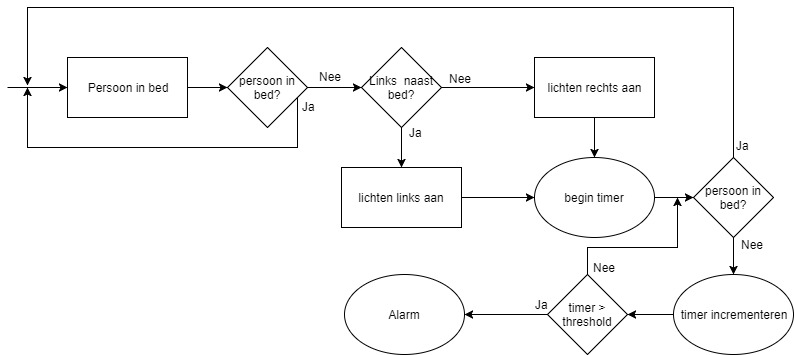
\includegraphics[scale=0.5]{HoogNiveauBlokDiagram}
	\caption{Werkingsschema op hoog niveau}
	\label{imgWeS}
\end{figure}
Dit onderzoek heeft als doel het ontwikkelen van een visiesysteem dat kan detecteren langs welke zijde pati\"enten uit bed stappen en kan meten hoelang de pati\"enten wegblijven. Als mogelijke uitbereiding kunnen we ook val detectie toevoegen. In figuur \ref{imgWeS} ziet u het werkingsschema op hoog niveau.
We beginnen links bovenaan. We gaan er vanuit dat er een persoon in het bed ligt. Vervolgens gaan we testen of er delen van het lichaam zich uit het bed bevinden. Indien er geen delen uit het bed zijn blijven we deze test herhalen. Indien er wel delen uit het bed zijn, gaan we kijken naar welke zijde. Vanaf het moment dat de persoon het bed heeft verlaten, begint er een teller te lopen. Elke keer gaan we de waarde van de teller vergelijken met een threshold. Dit zodat er een alarm gegenereerd wordt als een persoon te lang wegblijft. Als de persoon terug in het beeld komt, stopt de teller en bevinden we ons weer in de eerste toestand.

\section{IR camera}
\label{MRefIRC}
Voor de uitwerking van ons project maken we gebruik van een infrarood camera. Deze hebben we eerder al besproken in onze literatuurstudie \ref{refIRC}. We gebruiken deze camera omdat deze ter beschikking werd gesteld door het school en dit ons ook een logische keuze leek. Dit omdat de persoon door de infraroodbeelden al minder snel herkenbaar zijn op de beelden wat een zeer belangrijk deel zijn van de specificaties. In dit stuk tekst bespreken we eerst de camera die we gebruiken, namelijk de Seek Thermal Compact \ref{mRefSTh}, daarna bespreken we de plaatsing van de camera \ref{mRefSTP}. Andere types van camera zoals bijvoorbeeld een 3D-camera en een night vision camera of een andere IR camera kunnen natuurlijk ook gebruikt worden. Maar dit hebben we in dit onderzoek niet bestudeerd.

\subsection{Seek Thermal Compact}
\label{mRefSTh}

\begin{figure}[hbp]
	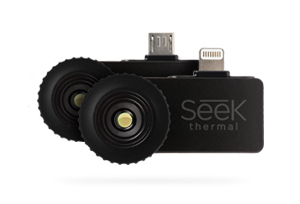
\includegraphics[scale=0.75]{SeekThermalCompac}
	\caption{Image of Seek Thermal Compact}
	\label{imgSTC}
\end{figure}
Dit is een zeer kleine camera die bedoeld is om te gebruiken met een Android smartphone of met een IPhone. U kan een afbeelding van de camera zien in figuur \ref{imgSTC} \cite{bibImgSTC}. Door de code die me beschikbaar is gesteld via eavise \cite{bibSTC} heb ik deze kunnen aansluiten op mijn computer en kan ik hiermee beelden binnen halen. Met deze camera maakte ik tevens testbeelden die we in onze code \ref{mrefCod} gebruiken.//In dit deel van de tekst bespreken we nog kort de specificaties van de camera \ref{mRefSTS} en maken we een berekening van hoe hoog we de camera moeten plaatsen om het volledige bed in het frame te krijgen \ref{mRefSTP}.

\subsubsection{Specificaties}
\label{mRefSTS}
De Seek Thermal Compact voor Android Systemen heeft volgende specificaties
\begin{itemize}
	\item $\mu$USB Thermal Camera for Android devices
	\item Werkt met de meeste Android toestellen die werken met 4.3 of hoger. (Op de website vind je een lijst met compatibele toestellen \cite{bibImgSTC}
	\item 206 * 156 Thermal Sensor
	\item 12 $\mu$ Pixel Pitch
	\item Vanadium Oxide Microbolometer
	\item Chalocogeninde Lens
	\item $36^{\circ}$ zicht
	\item Magnesium behuizing
	\item Lange golf infrarood 7.2 - 13 Microns
	\item  spectrom van -40 tot 330 °c
	\item <9Hz
	\item Bevat een waterdichte cover
	\item Model: UW-AAA
\end{itemize}
\cite{bibImgSTC}

\subsection {Plaatsing van de camera}
\label{mRefSTP}
Er zijn verschillende manieren. om de camera te plaatsen. Maar aangezien we het bed in de code coderen, willen we dat de positie van het bed hetzelfde blijft ten opzichte van de camera. Dit kunnen we doen door de camera via een constructie aan het bed te bevestigen. We weten de openingshoek van de camera. Dankzij deze kunnen we de nodige hoogte van de camera berekenen. We nemen de lengte van het bed (2m) als de bepalende factor voor de hoogte. Als laatst bepalen we ook de hoogte waarop we de camera moeten bevestigen als hij niet bevestigd wordt aan het bed maar op een afstand van het voeteneinde van het bed. Je mag natuurlijk altijd de camera hoger hangen dan de berekende hoogte, dan ga je meer van de omgeving kunnen zien.

\subsubsection{Camera recht boven hoofdeinde}
Op de afbeelding ziet u een schets van hoe de constructie er uit zo komen te zien \ref{imgCBB}.
\begin{figure}[hbp]
	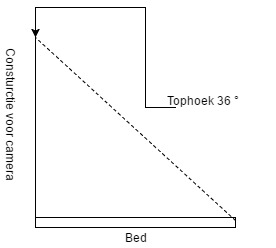
\includegraphics[scale=0.7]{CamBovenBed}
	\caption{Schets van camera recht boven bed}
	\label{imgCBB}
\end{figure}
De berekening is in dit geval heel eenvoudig. Het gaat hier over een rechthoekige driehoek. We kunnen de standaard sinus en cosinus regels hier gebruiken.
\begin{gather}
tan(\alpha) =\frac{o}{x}\\
tan(36) = \frac{2}{x} \\
\Rightarrow x = \frac{2}{tan(36)} = 2.75
\end{gather}
met
\begin{itemize}
	\item $\alpha$ is de openingshoek van de camera in uitgedrukt graden
	\item o is de lengte van het bed uitgedrukt in meter
	\item x is de gevraagde hoogte in meter
\end{itemize}

Uit de berekeningen blijkt dat de camera 2.75 meter boven het bed moet hangen. Dit is onmogelijk omdat de gemiddelde kamer ongeveer een 2.5 meter hoog is.

\subsubsection{Camera niet recht boven hoofdeinde}
\begin{figure}[hbp]
	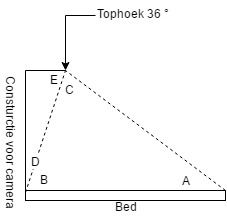
\includegraphics[scale=0.7]{CameraNietRechtBoven}
	\caption{Schets van camera niet recht boven bed}
	\label{imgCNRBB}
\end{figure}
Met deze berekening gaan we zien of het wel mogelijk is om een persoon volledig in het beeld te krijgen door de camera iets meer naar het voeten einde van het bed op te schuiven. Een schets ziet u in figuur \ref{imgCNRBB}. De drukletters in de figuur \ref{imgCNRBB} zijn de verschillende hoeken. Deze worden ook in de berekening gebruikt .Door te rekenen met hoeken in driehoeken en het gebruik van de sinusregels voor willekeurige- en rechthoekige driehoeken, kunnen we de gezochte hoogte berekenen. Alle hoeken worden uitgedrukt in graden en de lengtes in meter. Voor het horizontale gedeelte van de constructie nemen we een paar keer een andere waarde, zo kan u zien hoe de hoogte evolueert.
\begin{gather}
C=36\\
A+B+C=180 \\
E+D=90 \\
B+D=90 \\
\Rightarrow B=E
\frac{2}{sin(36)}=\frac{schuin}{sin(180-36-E)}\\
cos(E)=\frac{horizontaal}{schuin}\\
\Rightarrow cos(E)sin(144-E)=\frac{horizontaal*sin(36)}{2}\\
hoogte=tan(E)*horizontaal
\end{gather}
met:
\begin{description}
	\item[schuin] de schuine zijde in de driehoek (tussen B en C)
	\item[horizontaal] het horizontale stuk van de constructie
	\item[hoogte] de hoogte waarop de camera moet komen
\end{description}
Uit (3.10) berekenen we de hoek E door elke keer voor horizontaal een lengte in te vullen. Eens de hoek berekend is kunnen we gemakkelijk de hoogte berekenen via (3.11). Een overzicht van de berekende waarden, ziet u in tabel \ref{refTabCNRBB}. Uit deze waarden kunnen we besluiten dat het onmogelijk is om de camera in een normale ruimte aan het bed te bevestigen.
\begin{table}[hbp]
	\caption{Berekende waarden voor camera niet recht boven hoofdeinde}
	\begin{tabular}{|c|c|c|}
		\hline
		horizontaal & E & hoogte \\ \hline
		0.1 & 88 & 2.86 \\ \hline
		0.25 & 85 & 2.85 \\ \hline
		0.5 & 81 & 3.15 \\ \hline
		0.75 & 76 & 3.01 \\ \hline
		1 &  72 & 3.08 \\
		\hline
	\end{tabular}
	\label{refTabCNRBB}
\end{table}

\subsubsection{Camera niet bevestigd aan het bed}
In dit deeltje van de tekst bepalen we de nodige hoogte van de camera indien deze niet aan het bed bevestigd wordt, maar wel op een bepaalde afstand van het voeten einde van het bed. Een schets van de situatie vindt u in de afbeelding \ref{imgCNB}. 
\begin{figure}[hbp]
	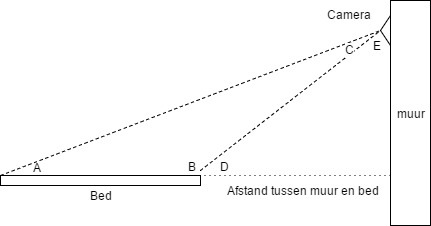
\includegraphics[scale=0.7]{CameraNietAanBed}
	\caption{Schets van camera niet bevestigd aan bed}
	\label{imgCNB}
\end{figure}
Net zoals bij de vorige berekening vindt u de namen van de hoeken terug in de afbeelding. Bij deze berekening nemen we aan dat de camera zelf geen dikte heeft. Dus de hoek E zit tussen de denkbeeldige lijn die de openingshoek van de camera weer geeft en de muur. Dit om de berekeningen iets eenvoudiger te houden. 

\begin{gather}
C=36\\
A+B+C=180 \\
B+D=180 \\
\Rightarrow A=D-36\\
\frac{2}{sin(36)}=\frac{schuin}{sin(D-36)}\\
cos(D)=\frac{horizontaal}{schuin}\\
\Rightarrow cos(D)sin(D-36)=\frac{horizontaal*sin(36)}{2}\\
hoogte=tan(D)*horizontaal
\end{gather}
met:
\begin{description}
	\item[schuin] de schuine zijde in de driehoek (tussen B en C)
	\item[horizontaal] de afstand tussen het bed en de muur
	\item[hoogte] de hoogte waarop de camera moet komen
\end{description}
Uit (3.18) berekenen we de hoek D door elke keer voor horizontaal een lengte in te vullen. Eens de hoek berekend is kunnen we gemakkelijk de hoogte berekenen via (3.19). Een overzicht van de berekende waarden, ziet u in tabel \ref{refTabCNB}.

\begin{table}[hbp]
	\caption{Berekende waarden camera niet aan bed bevestigd}
	\begin{tabular}{|c|c|c|}
		\hline
		horizontaal & D & hoogte \\ \hline
		0.25 & 84 & 2.37 \\ \hline
		0.5 & 77 & 2.16 \\ 
		\hline
	\end{tabular}
	\label{refTabCNB}
\end{table}

\subsubsection{Besluiten bij de berekeningen}
Uit de eerste twee berekeningen besluiten we dat het onmogelijk is om de gebruikte camera aan het bed te bevestigen en heel het bed te zien. Er zijn twee mogelijke oplossingen. We kunnen een andere camera nemen met een grotere openingshoek, of we kunnen de camera verder van het bed plaatsen zodat de benodigde hoogte kleiner gaat worden.\\
Uit de tweede berekening kunnen we besluiten dat het met de gebruikte camera wel mogelijk is om het volledige bed in de frame te krijgen. Als we de camera achter het bed aan de muur hangen. Uit de berekeningen blijkt dat hoe groter de afstand tot het bed, hoe minder hoog de camera moet komen te hangen.

\section{Code}
\label{mrefCod}
In dit deel bespreken we de code die we geschreven hebben. We gaan dit doen klasse per klasse. De code is geschreven in c++ en maakt voornamelijk gebruikt van openCV. De gebruikte code is terug te vinden op de cd die samen met de tekst wordt binnengebracht. De eerste besproken klasse is SaveImages \ref{mRefSIm}, deze wordt gebruikt om afbeeldingen op te slagen, de tweede klasse is GetImages \ref{mRefGIm}, deze gaat opgeslagen afbeeldingen uit het geheugen ophalen. De volgende klasse is de klasse Bed \ref{mRefBed} deze klasse wordt gebruikt om het bed te defini\"eren. De voorlaatste klasse is de belangrijkste klasse van ons project, namelijk de klasse Detect \ref{mRefDet},de laatste klasse DetectNotNormalized \ref{mRefDNN} is afgeleid van de Detect klasse, maar er zijn een paar kleine wijzigingen in gebeurd.\\ 
Buiten deze klassen zijn er ook verschillende testprogramma's geschreven, hierin staat telkens de main loop die de verschillende klassen met hun methodes gaat oproepen \ref{mRefTPr}.\\
Als laatste bespreken we ook nog de geschreven functies die niet tot een bepaalde klasse behoren \ref{MRefGFu}.

\subsection{SaveImages}
\label{mRefSIm}
Dit is de eerste klasse die we geschreven hebben. Het doel van deze klasse is het opslaan van een afbeelding. Deze klasse bevat in methode saveImage, deze heeft als argumenten, de afbeelding die opgeslagen wordt en het pad waar de afbeelding moet opgeslagen worden.  
Er kan ge\"evalueerd worden of het nodig is om deze klasse te behouden. Dit hangt af of men de beelden op een server wilt bijhouden. In de eerste fasen van het project is dit wel gemakkelijk, dan kan je eventueel nagaan waar er eventueel fouten gemaakt zijn. 
Het oorspronkelijk idee van deze klasse was dat er 's nachts beelden als wijze van experiment gemaakt kunnen worden die we dan overdag kunnen gebruiken.

\subsection{GetImages}
\label{mRefGIm}
Deze klasse is het tegenovergestelde van de vorige besproken klasse \ref{mRefSIm}. Deze klasse bevat wederom \'e\'en methode, namelijk saveImage. Deze methode heeft \'e\'en argument, het pad naar de afbeelding die we willen ophalen. De klasse geeft de gevraagde afbeelding terug.

\subsection{Bed}
\label{mRefBed}
In deze klasse maken we een bed object aan. Het bed object bevat 8 integers, dit zijn de co\"ordinaten van de x- en y- posities van de vier hoeken van het bed. We bepalen 1 keer per kamer de positie van het bed. Dit doordat op de infraroodbeelden nooit het bed te zien zal zijn. Deze klasse omvat drie constructoren en vier methodes, namelijk setValues, set ValuesImg, sidesOfBed en setValuesAuto.

\subsubsection{Constructoren}
Er zijn drie verschillende manieren om een bed object aan te maken. De eerste heeft geen argumenten, het tweede heeft acht integers als argumenten, dit zijn de x- en y- co\"ordinaten van de vier hoeken. Als laatste is er ook een constructor met een afbeelding en een integer als argument.

\paragraph{Geen argumenten}
Wanneer er een bed wordt aangemaakt zonder argumenten, wordt het bed in een punt in de linkerbovenhoek geplaatst dit door de methode setValues op te roepen met acht maal 0 als argumenten. Er wordt in de terminal het bericht geplaatst dat ze de methode setValue of setValuesImg van deze klasse nog moeten oproepen, om de juiste co\"ordinaten van de hoeken in te geven. 

\paragraph{Acht integers als argument}
Een bed object kan gemaakt worden met acht getallen als argument. Dit zijn de co\"ordinaten van de vier hoeken van het bed. De hoeken worden in wijzerzin meegegeven, beginnen bij de rechterbovenhoek van het bed. In deze constructor wordt de methode setValues (deze wordt later nog uitgebreider besproken) opgeroepen. De acht integers worden als argument met de methode oproep meegegeven. Het resultaat is een Bed object waarvan de vier hoeken de juiste co\"ordinaten hebben.

\paragraph{Afbeelding en integer als argument}
\begin{figure}[hbp]
	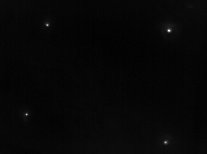
\includegraphics[scale=0.75]{SeekCamBed}
	\caption{Foto van het bed met kaarsjes op de hoeken}
	\label{imgCBe}
\end{figure}
Een bed object kan eveneens gemaakt worden door een afbeelding en een integer mee te geven. Om eenmalig de hoeken van het bed te bepalen, zonder dat je zelf moet gaan puzzelen op welke pixels net de hoeken liggen, gaan we op de hoeken van het bed een paar warmere objecten  te leggen. Dit kunnen bijvoorbeeld kaarsjes zijn. Maar alles wat warmer is als het bed werkt perfect. Voor de nauwkeurigheid raden we wel aan dat dit kleine objecten zijn. Hier trekken we dan met de camera een foto van. Een voorbeeld van dergelijke afbeelding vindt u in figuur \ref{imgCBe}. 

\subparagraph{integer is 0}
Dit is de eerste versie van de constructor. De meegegeven afbeelding, waarvan u een voorbeeld ziet in \ref{imgCBe}, wordt meegegeven aan de methode setValuesImg. Hoe deze methode precies werkt, bespreken we later. Het resultaat is een Bed object waar de vier hoekpunten de co\"ordinaten hebben waar voordien kaarsjes stonden.

\subparagraph{integer is niet 0}
Dit is de achteraf toegevoegde maar veel gebruiksvriendelijkere versie van de constructor. Het zelfde type van afbeelding wordt hier gebruikt. De locatie van de hoeken wordt automatisch bepaald. De afbeelding wordt meegegeven met de methode setValuesAuto. De werking hiervan wordt later uitgelegd.

\subsubsection{setValues}
De naam maakt duidelijk wat de bedoeling is van deze methode. We geven hier acht getallen mee. Dit zijn de co\"ordinaten van de vier hoekpunten van het bed. Deze worden dan opgeslagen in het bed object. De volgorde van de getallen in, in wijzerzin, beginnende bij de rechterbovenhoek van het bed. Verder geven we eerst de x-co\"ordinaat in gevolgd door de y-co\"ordinaat.

\subsubsection{setValuesImg}
Deze methode heeft als argument een afbeelding. Via het oproepen van de mouseCallBack functie die besproken wordt in \ref{MRefGFu} gaan we door het klikken op de lichtere punten van de afbeelding de verschillende waarden van de co\"ordinaten van de hoeken bepalen. Ook hier beginnen we met klikken op de rechterbovenhoek van het bed. 

\subsubsection{sidesOfBed}
Deze methode gaat aan de hand van de ingegeven punten de zijkanten van het bed defini\"eren aan de hand van een vergelijking van een rechte. Dit omdat je dan later kan zien wanneer een persoon over de rand stapt. Je moet hier geen argumenten meegeven. De functie geeft wel een vector terug met daarin de vier waarden, dit zijn de co\"effici\"enten van de twee vergelijkingen. We nemen aan dat een persoon enkel via de zijkanten uit een bed gaat stappen en niet langs bijvoorbeeld het hoofd- of voeteneinde.

\subsubsection{setValuesAuto}
Deze methode heeft als argument een afbeelding. Deze afbeelding is de zelfde als de afbeelding die reeds gebruikt werd in setValuesImg. De bedoeling van deze methode is dat hij in de gegeven afbeelding automatisch de vier hoeken van het bed gaat detecteren en deze gaat meegeven aan het bed object. Het is een soort van blobdetectie algoritme. Het algoritme kan wel enkel gebruikt worden in deze toepassing. De werking van deze methode wordt verduidelijkt via de flowchart, deze ziet u in figuur \ref{imgFCSVA}. Het werkingsprincipe is vrij eenvoudig. Je gaat de pixelwaarden vergelijken met een threshold. Als je een wit punt vind, hoort dit bij de hoeken. Maar doordat het warm object groter is dan \'e\'en pixel, ga je eerst nakijken of er niet al een punt uit de directe omgeving is opgeslagen in de vector. Als er nog geen buurpunt was opgeslagen wordt het punt opgeslagen in de vector. Als de volledige afbeelding is afgelopen, ga je zien welk punt het meest naar beneden staat. Dit is de linkeronderhoek van het bed. Vervolgens bereken je de afstanden tussen de punten en het onderste punt. Aan de hand van deze afstanden kan je bepalen welke co\"ordinaten bij welk hoekpunt horen.
\begin{figure}[hbp]
	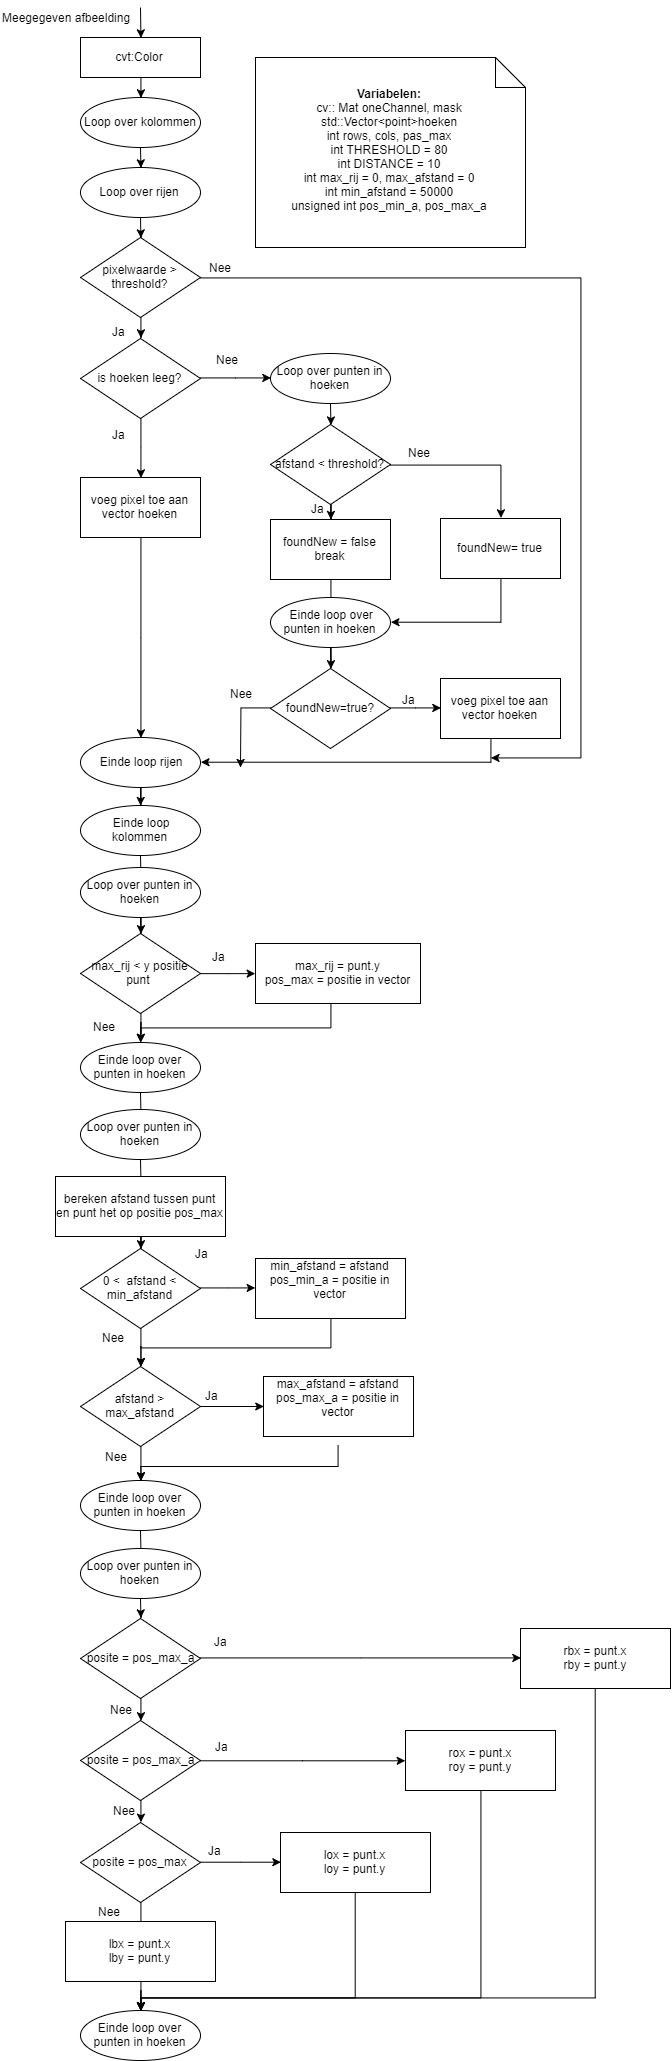
\includegraphics[scale=0.34]{FlowChart_setValuesAuto}
	\caption{Flowchart van de methode setValuesAuto}
	\label{imgFCSVA}
\end{figure}

\subsection{Detect}
\label{mRefDet}
In deze klasse worden de detectie van het uit het bed stappen gedaan. Om een object van de klasse Detect te maken, moet je een object van de klasse Bed toewijzen. De klasse Detect bevat twee constructoren. Deze worden eerst besproken. Vervolgens bespreken we de verschillende methodes van deze klasse. De eerste methode is createMask, de tweede is checkMovement, de volgende is checkBed, hierna is er ook nog de tempDifference methode, als voorlaatste is er de createMaskNew methode en om af te sluiten hebben we de erDil methode.

\subsubsection{Constructoren}
De klasse heeft 2 verschillende contructoren, namelijk een afbeelding als argument of acht integers als argument.

\paragraph{Afbeelding als argument}
De eerste constructor van de klasse heeft een afbeelding als argument. We  roepen de methode setValuesAuto van de klasse bed op. Zo krijgt het bed object van de klasse de juiste co\"ordinaten voor de hoekpunten. 

\paragraph{Acht integers als argument}
De tweede constructor heeft acht integers als argument. Met deze waarden wordt de methode setValues van het bed object opgeroepen.

\subsubsection{createMask}
\begin{figure}[hbp]
	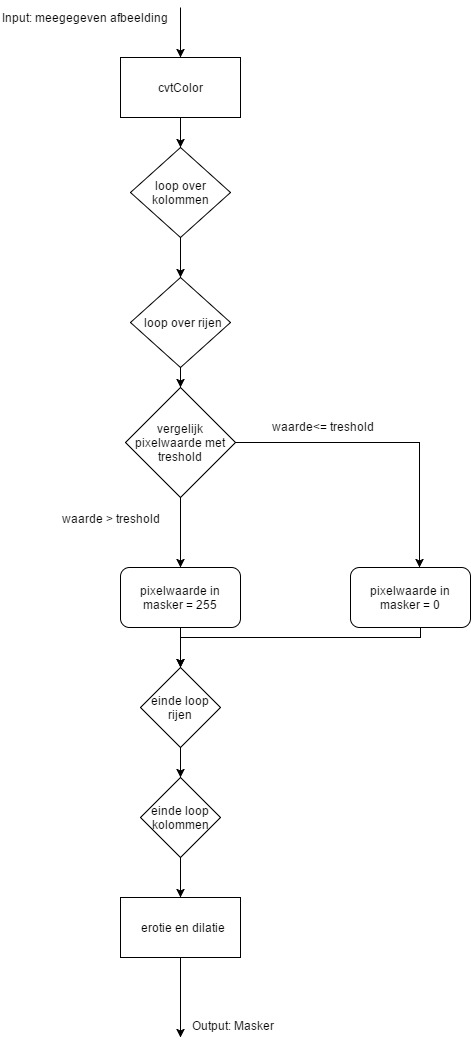
\includegraphics[scale=0.45]{FlowShart_createMask}
	\caption{Flowchart van de methode createMask}
	\label{imgFSCMa}
\end{figure}

Deze methode heeft als doel het maken van het masker. We leggen het werkingsprincipe van de methode uit aan de hand van een flowchart. Deze ziet u in figuur \ref{imgFSCMa}. Het principe is heel eenvoudig, als argument wordt er een afbeelding meegegeven. De afbeelding die we inlezen is 3 kanaal. Daarom zetten we de afbeelding eerst om naar een 1 kanaal afbeelding. Dit is de eerste rechthoek in onze flowchart.  Deze wordt vervolgens  pixel per pixel doorlopen. Als de waarde op de bewuste pixel groter is dan de threshold wordt de overeenkomende pixel in het masker wit gemaakt, De rest blijft zwart. Dit wordt ook gedaan zodat de persoon in de beelden onherkenbaar zou zijn. Het masker wordt terug gegeven. De door ons gebruikte drempelwaarde heeft een waarde van 180 gekregen. Nadat de rijen en kolommen zijn doorlopen wordt er erosie en dillatie toegepast, dit is het laatste rechthoekje in de figuur. Vervolgens wordt het masker terug gegeven.  Een voorbeeld van een meegegeven afbeelding en een teruggekregen masker ziet u in figuur \ref{imgCMa}.

\begin{figure}[hbp]
	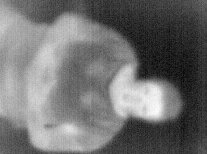
\includegraphics[scale=0.75]{EersteExperiment_img0}
	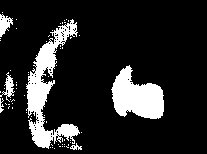
\includegraphics[scale = 0.75]{EersteExperiment_mask0}
	\caption{Voorbeeld van masker: (links) meegegeven afbeelding (rechts) verkregen masker}
	\label{imgCMa}
\end{figure}

\subsubsection{checkMovement}
Deze methode gaat 2 opeenvolgende frames vergelijken om te zien of het de moeite is om de volgende zwaardere berekeningen te doen. Indien er geen beweging is geweest, kan de persoon ook niet uit bed gestapt zijn, of eruit gevallen. Deze methode heeft als argument 2 opeenvolgende frames. Deze worden pixel per pixel vergeleken. Het aantal pixels waar er een verschillende waarde is wordt bijgehouden. Deze wordt vergeleken met een drempelwaarde. Indien het aantal verschillende pixels kleiner is dan de drempelwaarde, is er geen beweging geweest en wordt false terug gegeven. Indien er wel meer verschillende pixelwaarden zijn, heeft de persoon bewogen en wordt er true terug gegeven.

\subsubsection{checkBed}
\begin{figure}[hbp]
	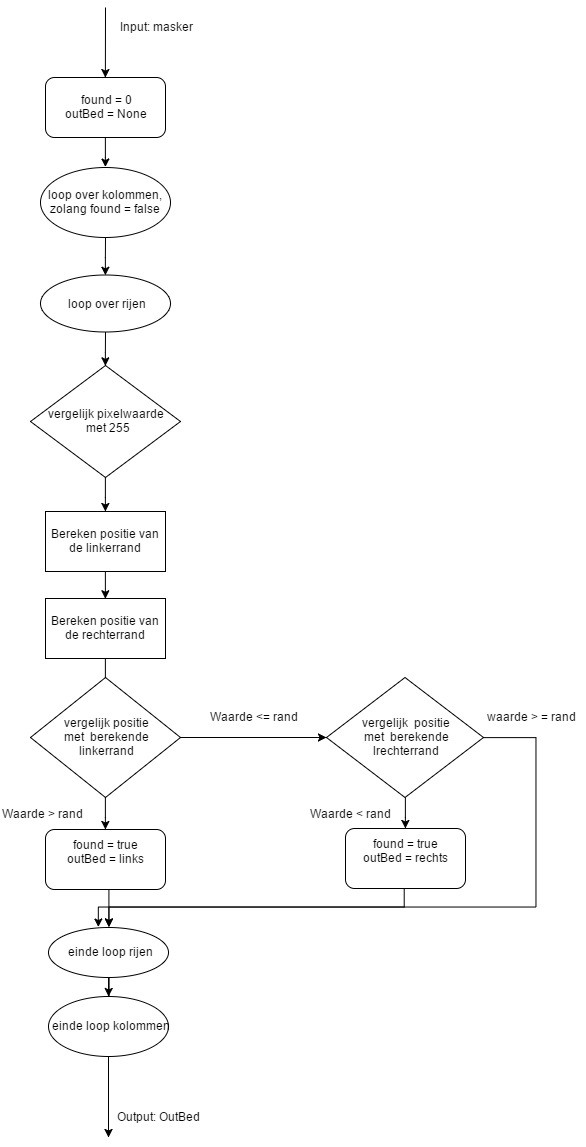
\includegraphics[scale=0.45]{FlowShart_checkBed}
	\caption{Flowchart van de methode checkBed}
	\label{imgFCCBe}
\end{figure}
Deze methode wordt verduidelijkt aan de hand van een flowchart. Deze vindt u terug in figuur \ref{imgFCCBe}. De methode checkBed heeft \'e\'en argument, namelijk een afbeelding. Als je deze methode oproept, geef je het masker mee dat door de methode createMask gemaakt werd. In deze methode gaat men kijken of er delen die door het masker aangeduid werden als pati\"ent uit het bed steken. \\
We gaan voor elke kolom kijken. Als er een witte pixel gevonden is, gaat men eerst bekijken waar deze licht ten opzichte van de linkse bedrand. Die kan je halen uit de vergelijkingen die bepaald worden door sidesOfBed in de klasse bed. Als de waarde groter is, dan is er daar een lichaamsdeel over de bed rand. Er wordt terug gegeven dat er links uit het bed gestapt wordt. Indien de waarde kleiner is gaat men vergelijken met de y-waarde van de rechter bed rand. Heeft de gevonden y waarde een grotere waarde dan die van de rechter bed rand, dan stapt de persoon langs rechts uit bed. Indien de y-waarde tussen de bedranden blijft, gebeurt er niets.

\subsubsection{tempDifference}
\begin{figure}[hbp]
	\includegraphics[scale=0.45]{FlowChart_TempDifference}
	\caption{Flowchart van de methode tempDifference}
	\label{imgFCTDi}
\end{figure}
Deze methode is toegevoegd na het uitvoeren van het tweede experiment \ref{ERefDUB} en het maken van onze conclusies hieruit \ref{ERefDBB}. Deze methode heeft veel weg van de checkMovement methode die we hierboven hebben besproken. Om de werking van de methode te verduidelijken, hebben we een flowchart toegevoegd in figuur \ref{imgFCTDi}. In deze methode berekenen we temporeel verschil zoals besproken bij voorgrond /achtergrond segmentatie \ref{refBET}. Er wordt een afbeelding teruggegeven waarbij alle pixels nul als waarde hebben, buiten de pixels waar de waarde niet hetzelfde is voor de twee opeenvolgende frames, die pixel heeft de waarde 255.Een voorbeeld van het resultaat, dat ik vanaf nu bewegingsMasker noem, vindt u in figuur \ref{imgBMa}. \\
Deze extra stap wordt gedaan om te vermijden dat warmere vlekken van de achtergrond verward worden met lichaamsdelen van een persoon.
\begin{figure}[hbp]
	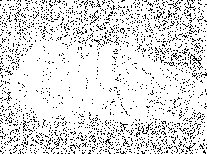
\includegraphics[scale=0.75]{bewegingsMatrix}
	\caption{Voorbeeld van een bewegingsmasker}
	\label{imgBMa}
\end{figure}

\subsubsection{createMaskNew}
\begin{figure}[hbp]
	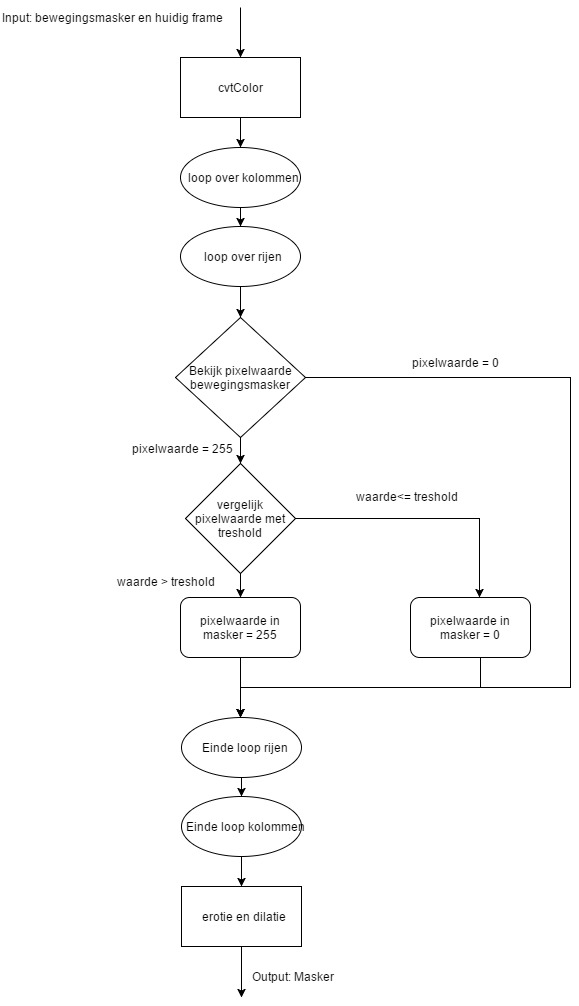
\includegraphics[scale=0.45]{FlowChart_createMaskNew}
	\caption{Flowchart van de methode createMaskNew}
	\label{imgFCCMN}
\end{figure}
Om het werkingsprincipe van deze methode te verduidelijken, hebben we een flowchart toegevoegd. Deze vindt u in figuur \ref{imgFCCMN}. Zoals u uit deze figuur en uit figuur \ref{imgFSCMa} kunt afleiden, lijkt deze methode op de reeds besproken methode createMask. Dit komt doordat dit een nieuwere, verbeterde versie is van createMask. Deze methode heeft twee argumenten, namelijk de huidige frame en het bewegingsmasker, dat als resultaat uit de methode tempDifference komt. We gaan opnieuw \'e\'en voor \'e\'en over alle pixels lopen en bekijken het bewegingsmasker, is de waarde voor de huidige pixel gelijk aan 255, dan bekijken we de meegegeven frame. Is de pixel waarde van de frame groter dan de threshold, dan wordt de pixelwaarde van het terug gegeven masker 255. Anders blijft de pixelwaarde nul. Voor we het berekende masker gaan terug geven gaan we nog eroderen en vervolgens dilleren, dit om de mogelijk kleine afwijkingen te elimineren, zodat er geen valse detecties gebeuren. Hiervoor gebruiken we de methode erDil die besproken wordt in de volgende paragraaf. Een voorbeeld van een masker dat terug gegeven wordt en het originele frame vindt u terug in figuur \ref{imgCMN}.
\begin{figure}[hbp]
	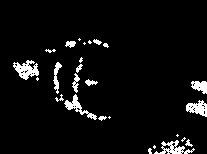
\includegraphics[scale=0.65]{MaskMetDif}
	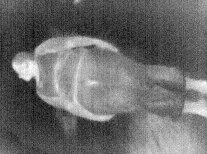
\includegraphics[scale=0.65]{ImgMetDif}
	\caption{Frame en masker gemaakt met methode createMaskNew}
	\label{imgCMN}
\end{figure} 
 
 \subsubsection{erDil}
Deze methode heeft twee argumenten. De eerste is de afbeelding waarop de erosie en dillatie toegepast moet worden. Het tweede is de grootte van de matrix gebruikt voor het eroderen en dilleren. Hoe groter de waarde, hoe meer details er van de afbeelding verdwijnen. Nadat de erosie en dillatie, wat men ook wel openen noemt, is toegepast wordt de resultaatafbeelding terug gegeven. 
 
 \subsubsection{tempDifferenceNew}
Deze methode is een verbetering van het bewegingsmasker. Deze methode heeft als doel een oplossing te bieden voor het probleem van de restwarmte. We gaan ook hier weer twee opeenvolgende frames met elkaar vergelijken. Als de pixelwaarde van het huidige frame min de pixelwaarde van de vorige frame groter is, dan wordt de pixelwaarde van het bewegingsmasker 255. Waarom enkel als de waarde groter is? Omdat de persoon normaal het warmste deel van het beeld moet zijn. Hierdoor zal dus de beweging van de persoon gepaard gaan met het stijgen van de pixelwaarde. De dalende pixelwaarden zijn bijvoorbeeld het afkoelen van het bed nadat de persoon eruit is gestapt en hebben we verder niet meer nodig.
 
 \subsection{DetectNotNotmalized}
 \label{mRefDNN}
Deze klasse is afgeleid van de eerder besproken Detect \ref{mRefDet} klasse. Deze klasse is gemaakt om te werken met live beelden en zonder normalisatie. Deze klasse heeft \'e\'en methode. Namelijk createMask.
 
 \subsubsection{createMask}
 Deze methode is ongeveer het zelfde als de eerder verklaarde gelijknamige methode. Het grootste verschil is dat doordat je met live beelden werkt je de cvtColor stap niet nodig hebt. Het doel is nog altijd het zelfde, namelijk het cre\"eren van een masker dat wit is op de plaatsten waar er een persoon gedetecteerd wordt en de overige pixels zwart zijn. Voor deze methode is er geen nieuwe flowchart toegevoegd. U kan kijken naar die van createMask van de klasse Detect, figuur \ref{imgFSCMa}. U dient dus enkel de cvtColor stap over te slaan. 
 
\subsection{Gebruikte functies}
\label{MRefGFu}
Buiten de gebruikte klassen en hun methoden, is er eveneens een functie die tot de namespace LibSeek behoort.

\subsubsection{MouseCallBack}
Deze functie wordt bijvoorbeeld opgeroepen in de constructor van Bed als je deze oproept met een afbeelding als argument. De functie gaat de punten waarop geklikt wordt met de linkermuisknop opslagen in een vector. Door een klik met de rechtermuisknop, wordt het laatste punt in de vector verwijdert. Door op enter te klikken wordt de functie be\"eindigd. 

\subsection{Test Programma's}
\label{mRefTPr}
Er zijn verschillende testprogramma's geschreven. Dit telkens om aparte klassen en hun methodes te testen en eventuele optimalisaties toe te passen. We werken met zoveel verschillende test programma's omdat we het project stap voor stap hebben opgebouwd. We zijn zeer eenvoudig begonnen met het opslagen en ophalen van afbeeldingen. Vervolgens hebben we eerst een masker gemaakt, daarna zijn we begonnen met het detecteren van bewegingen, het aanmaken van bedobjecten. Daarna zijn we verschillende methoden voor detectie van uit bed stappen afgegaan en hebben deze getest. Per afgewerkte fase is er telkens een ander testprogramma.

\subsection{Uiteindelijke programma's}
\subsubsection{saveBed}
saveBed is het programma dat we hebben gemaakt om het frame van het bed op te slaan. In dit programma gaan we maar \'e\'en frame van de Libseek Thermal camera ophalen. Dit frame wordt opgeslagen in de speciaal aangemaakte map voor de bedden. Je moet dit programma niet dagelijks laten lopen. Je moet dit enkel doen als de camera of het bed verplaatst is geweest, of er reden is om te geloven dat de opgeslagen hoekpunten van het bed niet correct zijn. Natuurlijk moeten de warme objecten op voorhand op de hoekpunten geplaatst worden. Dit programma maakt gebruik van de klasse SaveImage en haar methode.

\subsection{Programma} 
Programma is de laatst werkende versie van het programma en al zijn functionaliteiten. Er wordt gebruik gemaakt van alle bovenstaande klassen. De gebruikten methoden varieerden gedurende de verschillende experimenten. Een bespreking van de verschillende gebruikte methoden vindt u terug in het volgende hoofdstuk \ref{ERef}.
